% !TeX document-id = {66b2d4b6-7613-4c19-b40c-a50fc00d38ff}
% !TeX program = lualatex
% !BIB program = biber
% Lualatex is important to render TTF fonts; with pdflatex it's just the regular one
% ratio 16:9 -- https://tex.stackexchange.com/questions/14336/

% compile two versions, inspired by https://tex.stackexchange.com/a/1501
% use the script "compile-pdf.sh"
\newif\ifhandout
% if flags.tex does not exist, create an empty file to be able to compile in TeXstudio
\input{flags}

\ifhandout
\documentclass[12pt,aspectratio=169,handout]{beamer}
\else
\documentclass[12pt,aspectratio=169]{beamer}
\fi

% adjust for 16:9
% https://tex.stackexchange.com/questions/354022/modifying-the-margins-of-all-slides-in-beamer
\setbeamersize{text margin left=0.3cm,text margin right=4.5cm} 

%\usepackage{xcolor}

% use Metropolis as the basis theme
\usetheme[subsectionpage=progressbar]{metropolis}
% blocks with background globally
\metroset{block=fill}

% ------- Paderborn specifics ----------
\usepackage{fontspec}
%\setsansfont{karla} % looked bad, too fat
\setsansfont{Segoe UI} % looks OK-ish

% Paderborn color scheme
\definecolor{UPBUltraBlue}{RGB}{0, 37, 170}

\setbeamercolor{frametitle}{bg=white, fg=UPBUltraBlue}

% name in footer
\setbeamertemplate{frame numbering}{Prof.\ Dr.\ Ivan Habernal ~ | ~ \insertframenumber }

% adjust the background to be completely white
\setbeamercolor{background canvas}{bg=white}

% add Paderborn logo at each slide
% actually not -- it's just eating up space
%\addtobeamertemplate{frametitle}{}{%
	%\begin{tikzpicture}[remember picture,overlay]
	%	\node[anchor=north east,yshift=2pt] at (current page.north east) {
\includegraphics[height=0.9cm]{img/UPB_Logo_ENG_coloured_RGB}};
	%\end{tikzpicture}
	%}

% show TOC at every section start
\AtBeginSection{
	\frame{
		\vspace{2em}
		\sectionpage
		\hspace*{2.2em}\begin{minipage}{10cm}
			\tableofcontents[currentsection]
		\end{minipage}
		% we need the logo to show up here as well
		\begin{tikzpicture}[remember picture,overlay]
			\node[anchor=north east,yshift=2pt] at (current page.north east) {
\includegraphics[height=0.9cm]{img/UPB_Logo_ENG_coloured_RGB}};
		\end{tikzpicture}
	}
}
% ------- end of Paderborn specifics ----------


% typeset mathematics on serif
\usefonttheme[onlymath]{serif}

% better bibliography using biber as backend
\usepackage[natbib=true,backend=biber,style=authoryear-icomp,maxbibnames=30,maxcitenames=9,uniquelist=false,giveninits=true,doi=false,url=false,dashed=false,isbn=false]{biblatex}
% shared bibliography
\addbibresource{../nlpwdl-bibliography.bib}
% disable "ibid" for repeated citations
\boolfalse{citetracker}



\usepackage{xspace}


% for derivatives, https://tex.stackexchange.com/a/412442
\usepackage{physics}

\usepackage{tikz}
\usetikzlibrary{matrix, positioning}
\usetikzlibrary{angles,quotes} % for angles
\usetikzlibrary{backgrounds} % background
\usetikzlibrary{decorations.pathreplacing} % curly braces
\usetikzlibrary{calligraphy}
\usetikzlibrary{calc} % for neural nets

% for plotting functions
\usepackage{pgfplots}
\usepgfplotslibrary{dateplot}

% sub-figures
\usepackage{caption}
\usepackage{subcaption}

% book tabs
\usepackage{booktabs}


% argmin, argmax
\usepackage{amsmath}
\DeclareMathOperator*{\argmax}{arg\!\max}
\DeclareMathOperator*{\argmin}{arg\!\min}
% softmax
\DeclareMathOperator*{\softmax}{soft\!\max}
% Mask
\DeclareMathOperator*{\mask}{mask}

% bold math
\usepackage{bm}

% for \mathclap
\usepackage{mathtools}

% algorithms
\usepackage[noend]{algpseudocode}


% for neurons and layers in tikz
\tikzset{
	neuron/.style={draw, rectangle, inner sep=2pt, minimum width=0.75cm, fill=blue!20},
	param/.style={draw, rectangle, inner sep=2pt, minimum width=0.75cm, fill=green!20},
	constant/.style={draw, rectangle, inner sep=2pt, minimum width=0.75cm, fill=black!15},
	% for citation nodes right top
	ref/.style={anchor = north east, text width=7.8cm, yshift=-1.3cm, xshift=-0.2cm, scale=0.5},
	state/.style={rectangle, inner sep=2pt, minimum width=0.75cm, fill=black!5},
}

% added in lecture 10
\tikzset{
	mtx/.style={
		matrix of math nodes,
		left delimiter={[}, right delimiter={]}
	},
	hlt/.style={opacity=0.1, line width=4 mm, line cap=round},
	hltr/.style={opacity=0.5, rounded corners=2pt, inner sep=-1pt}
}

% for strike-through text (added in Lecture 06)
\usepackage[normalem]{ulem}

% added in Lecture 7
% RNN
\DeclareMathOperator*{\rnn}{RNN}
% RNN star
\DeclareMathOperator*{\rnnstar}{RNN^{*}}
% bi-RNN
\DeclareMathOperator*{\birnn}{biRNN}


% added in Lecture 9
\usetikzlibrary{fit} % for hightligting by calling "fit"

% algorithms
\usepackage[noend]{algpseudocode}


\title{Natural Language Processing with Deep Learning}
\subtitle{Lecture 11 -- Text generation 4: Decoder-only models and GPT}
\date{December 22, 2023}
\author{Prof.\ Dr.\ Ivan Habernal}
\institute{Natural Language Processing Group 
	\hfill 
\includegraphics[height=1.4cm]{img/UPB_Logo_ENG_coloured_RGB} \\
	Paderborn University \\
	We focus on Trustworthy Human Language Technologies \hfill \texttt{www.trusthlt.org} }

\begin{document}

\maketitle

\begin{frame}{Motivation}

We introduced BERT, a powerful transformer model for learning contextualized token embeddings

BERT can be used for
\begin{itemize}
	\item text classification (one sequence, two concatenated sequences)
	\item sequence labeling (classify each token, e.g., NER, POS)
\end{itemize}

	
\end{frame}


\begin{frame}{Transformer encoder (BERT)}
	
	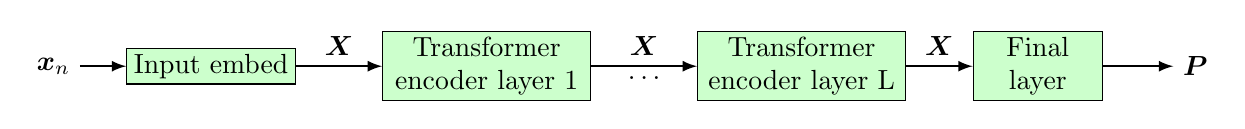
\begin{tikzpicture}
		
		\node (x) {$\bm{x}_n$};
		
		\node (emblayer) [param, right of=x, text centered, text width=2cm, xshift=1cm] {Input embed};
		
		%\node (X) [right of=emblayer, xshift=1cm] {$\bm{X}$};
		
		\node (trlayer1) [param, right of=emblayer, text centered, text width=2.5cm, xshift=2.5cm] {Transformer encoder layer 1};
		
		\node (trlayerN) [param, right of=trlayer1, text centered, text width=2.5cm, xshift=3cm] {Transformer encoder layer L};
		
		\node (finallayer) [param, right of=trlayerN, text centered, text width=1.5cm, xshift=2cm] {Final layer};
		
		\node (out) [right of=finallayer, xshift=1cm] {$\bm{P}$};
		
		\begin{scope}[thick, black, ->, >=latex]
			\draw (x) -- (emblayer);
			\draw (emblayer) -- (trlayer1) node [midway, above] {$\bm{X}$};
			\draw (trlayer1) -- (trlayerN) node [midway, above] {$\bm{X}$} node [midway, below] {$\ldots$};
			\draw (trlayerN) -- (finallayer) node [midway, above] {$\bm{X}$};
			\draw (finallayer) -- (out);
		\end{scope}	
	\end{tikzpicture}
	
	\vspace{4em}
	For each input token, BERT produces contextualized word embeddings
	
\end{frame}	


\begin{frame}{Motivation}
	

Although BERT is pre-trained with masked-language modeling, it is \textbf{not designed to generate text} by predicting the next token

Why?
\pause

We mask random tokens from the sequence and perform self-attention over past and future tokens

\bigskip

Can we use a transformer as a `true' language model, aka.\ to conditionally generate text?
	
\end{frame}

\begin{frame}{misc}

Bottom-up masking


Recap single-query attention with softmax

Show what needs to happen if you want to predict the last token

The last two tokens

On the full matrix



\begin{tikzpicture}[overlay, remember picture] 
	\node at (current page.north east)[ref] {\fullcite{Radford.et.al.2018.GPT1.report} \par};
\end{tikzpicture}

\end{frame}



\begin{frame}{Rel works}
	
Liu et al. Transformer (referred from GPT1 paper)

\begin{tikzpicture}[overlay, remember picture]
	\node at (current page.north east)[ref] {\fullcite{Liu.et.al.2018.ICLR} \par};
\end{tikzpicture}

	
\end{frame}



\begin{frame}{Recap: Single unmasked self-attention head (BERT)}
	
	\begin{tikzpicture}
		
		\node (X) {$\bm{X}$};
		
		\node (query) [param, right of=X, text centered, text width=2.2cm, xshift=2cm, yshift=1.6cm] {Linear layer (query)};
		
		\node (key) [param, right of=X, text centered, text width=2.2cm, xshift=2cm, yshift=0cm] {Linear layer (key)};
		
		\node (value) [param, right of=X, text centered, text width=2.2cm, xshift=2cm, yshift=-1.6cm] {Linear layer (value)};
		
		\node (scaled) [neuron, right of=key, text centered, text width=1.5cm, xshift=2.5cm, yshift=1cm] {Scaled dot product};
		
		\node (softmax) [neuron, right of=scaled, text centered, text width=1.8cm, xshift=1.6cm] {Softmax (row)};
		
		\node (matmul) [neuron, right of=softmax, text centered, text width=1.5cm, xshift=1.5cm] {Matmul $\bm{\tilde{S}}\bm{V}$};
		
		\node (out) [right of=matmul, xshift=1cm] {$\bm{Y}^h$};		
		
		\begin{scope}[thick, black, ->, >=latex]
			\draw (x) edge[out=0,in=180] (query);
			\draw (x) edge[out=0,in=180] (key);
			\draw (x) edge[out=0,in=180] (value);
			%			\draw (x) -- (sum1);
			\draw (query) edge[out=0,in=170] (scaled) node [right of=query, xshift=0.5cm, yshift=0.4cm] {$\bm{Q}$};
			\draw (key) edge[out=0,in=190] (scaled) node [right of=key, xshift=0.5cm, yshift=0.4cm] {$\bm{K}$};
			\draw (value) edge[out=0,in=210] (matmul) node [right of=value, xshift=0.5cm, yshift=0.6cm] {$\bm{V}$};
			\draw (scaled) -- (softmax) node [midway, above] {$\bm{S}$};
			\draw (softmax) -- (matmul) node [midway, above] {$\bm{\tilde{S}}$};
			
			%			\draw (norm1) -- (sum2)  node [near start, above] {$\bm{X}$};
			%			\draw (norm1) edge[out=0,in=180] (mlp);
			%			\draw (mlp) edge[out=0,in=270] (sum2) node [right of=mlp, xshift=0.3cm, yshift=0cm] {$\bm{X}$};
			%			\draw (sum2) -- (norm2) node [midway, above] {$\bm{X}$};
			\draw (matmul) -- (out);
		\end{scope}	
	\end{tikzpicture}
	
\end{frame}


\begin{frame}{Recap: Bidirectional / unmasked self-attention}
	
	\begin{minipage}[t][10cm][t]{15cm}
		
		Input: $\bm{X} \in \mathbb{R}^{\ell_{\text{x}} \times d_{\text{x}}}$, vector representations of the sequence of length $\ell_{\text{x}}$
		
		Output: $\bm{\tilde{V}} \in \mathbb{R}^{\ell_{\text{x}} \times d_{\text{out}}}$, updated vector representations of tokens in $\bm{X}$
		
		Params $\bm{\mathcal{W}_{qkv}}$: $\bm{W_q}, \bm{W_k} \in \mathbb{R}^{d_\text{x} \times d_\text{attn}}$, $\bm{b_q}, \bm{b_k} \in \mathbb{R}^{d_\text{attn}}$, $\bm{W_v} \in \mathbb{R}^{d_\text{x} \times d_\text{out}}$, $ \bm{b_v} \in \mathbb{R}^{d_\text{out}}$
		
		\begin{algorithmic}[1]
			\Function{Attention}{$\bm{X} ; \bm{\mathcal{W}_{qkv}}$}
			\State $\bm{Q} \gets \bm{X} \bm{W_q} +_{\text{(rows)}} \bm{b_q}$
			\Comment{Query $\in \mathbb{R}^{\ell_{\text{x}} \times d_{\text{attn}}}$}
			\State $\bm{K} \gets \bm{X} \bm{W_k} +_{\text{(rows)}} \bm{b_k}$
			\Comment{Key $\in \mathbb{R}^{\ell_{\text{x}} \times d_{\text{attn}}}$}
			\State $\bm{V} \gets \bm{X} \bm{W_v} +_{\text{(rows)}} \bm{b_v}$
			\Comment{Value $\in \mathbb{R}^{\ell_{\text{x}} \times d_{\text{out}}}$}
			
			\State $\bm{S} \gets \frac{1}{\sqrt{d_{\text{attn}}}} (\bm{Q} \bm{K}^\top)$
			\Comment{Scaled score $\in \mathbb{R}^{\ell_{\text{x}} \times \ell_{\text{x}}}$}
			
			\State \Return $\bm{\tilde V} = \softmax_{\text{row}}(\bm{S}) \bm{V}$
			
			\EndFunction
		\end{algorithmic}
		
	\end{minipage}
\end{frame}


\begin{frame}{Recap: Basic single-query attention}
	
	\begin{minipage}[t][10cm][t]{15cm}
		
		Input: $\bm{e} \in \mathbb{R}^{d_\text{in}}$, vector representation of the current token
		
		Input: $\bm{e}_t \in \mathbb{R}^{d_\text{in}}$, vector representations of the context tokens $t \in [T]$
		
		Output: $\bm{\tilde v} \in \mathbb{R}^{d_\text{out}}$, vector representation of the token and context combined
		
		Params: $\bm{W_q}, \bm{W_k} \in \mathbb{R}^{d_\text{in} \times d_\text{attn}}$, $\bm{b_q}, \bm{b_k} \in \mathbb{R}^{d_\text{attn}}$,
		$\bm{W_v} \in \mathbb{R}^{d_\text{in} \times d_\text{out}}$, $ \bm{b_v} \in \mathbb{R}^{d_\text{out}}$
		
		\begin{algorithmic}[1]
			\Function{Basic single-query attention}{}
			%\KwIn{}
			%\KwOut{$\v{\tilde v}∈ℝ^{d_\t{out}}$, vector representation of the token and context combined.}
			%\KwParam{$\m{W_q}, \m{W_k}∈ℝ^{d_\t{attn}×d_\t{in}}$, $ \v{b_q}, \v{b_k}∈ℝ^{d_\t{attn}}$, the query and key linear projections.}
			%\KwParam{$\m{W_v}∈ℝ^{d_\t{out}×d_\t{in}}$, $ \v{b_v}∈ℝ^{d_\t{out}}$, the value linear projection.}
			\State $\bm{q} \gets \bm{e} \bm{W_q} + \bm{b_q}$
			\Comment{Query linear projection}
			\For{$t \in [T]$}
			\State $\bm{k_t} \gets \bm{e_t} \bm{W_k} + \bm{b_k}$
			\Comment{Key linear projection}
			\State $\alpha_{t} = \frac{
				\exp(\bm{q} \cdot \bm{k_t} / \sqrt{d_{\text{attn}}})
			}{
				\sum_{u = 1}^{T}\exp(\bm{q} \cdot \bm{k_u} / \sqrt{d_{\text{attn}}})
			}$
			\Comment{Softmax over scaled dot products, $\alpha_{t} \in (0,1)$}
			\State $\bm{v_t} \gets \bm{e_t} \bm{W_v} + \bm{b_v}$
			\Comment{Value linear projection}
			\EndFor
			\State \Return $\bm{\tilde v} = \sum_{t=1}^T \alpha_t \bm{v}_t$
			\EndFunction
		\end{algorithmic}
		
	\end{minipage}
\end{frame}


\begin{frame}{Example: Basic single-query unmasked attention}

We are at position 2, our query $\bm{q} = (11, 12)$ and keys
$\bm{k_1} = (1, 2) \qquad \bm{k_2} = (4, 5) \qquad \bm{k_3} = (7, 8)$
$$
\bm{q} = \begin{pmatrix}
	11 & 12
\end{pmatrix}
\quad
\bm{K}^\top =
\begin{pmatrix}
1 & 4 & 7 \\
2 & 5 & 8 \\
\end{pmatrix}
\quad
$$
Dot products:

$\bm{q} \cdot \bm{k_1} = (11, 12) \cdot (1, 2) = 11 + 24 = 35$
$\bm{q} \cdot \bm{k_2} = (11, 12) \cdot (4, 5) = 44 + 60 = 104$
$\bm{q} \cdot \bm{k_3} = (11, 12) \cdot (7, 8) = 77 + 96 = 173$

Raw scores = $(35, 104, 173)$, after softmax (no scaling) $\bm{\alpha} = (0.000\ldots, 0.000\ldots, 0.999\ldots)$

Value at pos 3 most weight (from the future)



\end{frame}


\begin{frame}{We want to attend only to previous tokens}
	
For 4 tokens:

At position 1 we should not attend to token 2, 3, and 4

At position 2 we should not attend to token 2 and 3

At position 3 we should not attend to token 4

At position 4 we can attend to all of them
$$
\text{Raw associations } =
\begin{pmatrix}
11 & 12 & 13 & 14 \\
21 & 22 & 23 & 24 \\
31 & 32 & 33 & 34 \\
41 & 42 & 43 & 44 \\
\end{pmatrix}
$$
We want to assign zero probability (using softmax) to "future" tokens
\end{frame}


\begin{frame}{We want to attend only to previous tokens}
\begin{small}
\vspace{-2em}
	$$
	\text{Raw associations } =
	\begin{pmatrix}
		11 & 12 & 13 & 14 \\
		21 & 22 & 23 & 24 \\
		31 & 32 & 33 & 34 \\
		41 & 42 & 43 & 44 \\
	\end{pmatrix}
	$$
	Assign zero probability (using softmax) to "future" tokens
\end{small}

	\begin{algorithmic}[1]

	\For{$t \in [T]$}
	\State $\bm{k_t} \gets \ldots$
	\State $\alpha_{t} = \frac{
		\exp(\bm{q} \cdot \bm{k_t} )
	}{
		\sum_{u = 1}^{t}\exp(\bm{q} \cdot \bm{k_u} )
	}$
	\Comment{Only until $t$}
	\For{$i \in (t+1, T)$}
	\State $\alpha_i = 0$
	\Comment{Zero-out rest}
	\EndFor
	\State $\bm{v_t} \gets \ldots$
	\EndFor
	\State \Return $\bm{\tilde v} = \sum_{t=1}^T \alpha_t \bm{v}_t$

\end{algorithmic}


\end{frame}


\begin{frame}{Avoid for-loops!}
For each row $\bm{s}$ from the raw associations

\begin{algorithmic}[1]
	\State $\alpha_{t} = \frac{
		\exp(\bm{s}_t )
	}{
		\sum_{u = 1}^{t}\exp(\bm{s}_u )
	}$
	\For{$i \in (t+1, T)$}
	\State $\alpha_i = 0$
	\EndFor	
\end{algorithmic}

How to vectorize this operation?

\pause

Replace input from  $t + 1$ onwards with $-\infty$
\begin{small}
	$$
	\text{Raw associations "masked" } =
	\begin{pmatrix}
		11 & -\infty & -\infty & -\infty \\
		21 & 22 & -\infty & -\infty \\
		31 & 32 & 33 & -\infty \\
		41 & 42 & 43 & 44 \\
	\end{pmatrix}
	$$
	Assigns zero probability (using softmax) to "future" tokens
\end{small}



\end{frame}




\begin{frame}{Uni-directional masking for self-attention}

For $t_z, t_x \in [\ell_x]$
$$
\mask[t_x, t_z] =
 \begin{cases}
	1       & \quad \text{if } t_z \leq t_x \\
	0  & \quad \text{otherwise }
\end{cases}
$$


Example for $\ell_x = 4$
$$
\begin{pmatrix}
1 & 0 & 0 & 0 \\
1 & 1 & 0 & 0 \\
1 & 1 & 1 & 0 \\
1 & 1 & 1 & 1 \\
\end{pmatrix}
$$

\end{frame}


\begin{frame}{Left-to-right masked self-attention}
	
	\begin{minipage}[t][10cm][t]{15cm}
		
		Input: $\bm{X} \in \mathbb{R}^{\ell_{\text{x}} \times d_{\text{x}}}$, vector representations of the sequence of length $\ell_{\text{x}}$
		
		Output: $\bm{\tilde{V}} \in \mathbb{R}^{\ell_{\text{x}} \times d_{\text{out}}}$, updated vector representations of tokens in $\bm{X}$
		
		Params $\bm{\mathcal{W}_{qkv}}$: $\bm{W_q}, \bm{W_k} \in \mathbb{R}^{d_\text{x} \times d_\text{attn}}$, $\bm{b_q}, \bm{b_k} \in \mathbb{R}^{d_\text{attn}}$, $\bm{W_v} \in \mathbb{R}^{d_\text{x} \times d_\text{out}}$, $ \bm{b_v} \in \mathbb{R}^{d_\text{out}}$
		
		\begin{algorithmic}[1]
			\Function{Attention}{$\bm{X} ; \bm{\mathcal{W}_{qkv}}$}
			\State $\bm{Q} \gets \bm{X} \bm{W_q} +_{\text{(rows)}} \bm{b_q}$
			\Comment{Query $\in \mathbb{R}^{\ell_{\text{x}} \times d_{\text{attn}}}$}
			\State $\bm{K} \gets \bm{X} \bm{W_k} +_{\text{(rows)}} \bm{b_k}$
			\Comment{Key $\in \mathbb{R}^{\ell_{\text{x}} \times d_{\text{attn}}}$}
			\State $\bm{V} \gets \bm{X} \bm{W_v} +_{\text{(rows)}} \bm{b_v}$
			\Comment{Value $\in \mathbb{R}^{\ell_{\text{x}} \times d_{\text{out}}}$}
			
			\State $\bm{S} \gets \frac{1}{\sqrt{d_{\text{attn}}}} (\bm{Q} \bm{K}^\top)$
			\Comment{Scaled score $\in \mathbb{R}^{\ell_{\text{x}} \times \ell_{\text{x}}}$}

			\ForAll{$t_z, t_x \in [T] $}
			\If{$\neg \mask[t_x, t_z]$}
				 $\bm{S}[t_x, t_z] \gets - \infty$
	 			\Comment{Causal masking}
			\EndIf
			\EndFor
			\State \Return $\bm{\tilde V} = \softmax_{\text{row}}(\bm{S}) \bm{V}$
			
			\EndFunction
		\end{algorithmic}
		
	\end{minipage}
\end{frame}



\begin{frame}{Single masked self-attention head (GPT)}
	
	\begin{tikzpicture}
		
		\node (X) {$\bm{X}$};
		
		\node (query) [param, right of=X, text centered, text width=2.2cm, xshift=1.7cm, yshift=1.6cm] {Linear layer (query)};
		
		\node (key) [param, right of=X, text centered, text width=2.2cm, xshift=1.7cm, yshift=0cm] {Linear layer (key)};
		
		\node (value) [param, right of=X, text centered, text width=2.2cm, xshift=1.7cm, yshift=-1.6cm] {Linear layer (value)};
		
		\node (scaled) [neuron, right of=key, text centered, text width=1.5cm, xshift=2cm, yshift=1cm] {Scaled dot product};
		
		\node (mask) [neuron, right of=scaled, text centered, text width=1.5cm, xshift=1.3cm] {Masked};
		
		\node (softmax) [neuron, right of=mask, text centered, text width=1.8cm, xshift=1.4cm] {Softmax (row)};
		
		\node (matmul) [neuron, right of=softmax, text centered, text width=1.5cm, xshift=1.5cm] {Matmul $\bm{\tilde{S}}\bm{V}$};
		
		\node (out) [right of=matmul, xshift=1cm] {$\bm{Y}^h$};		
		
		\begin{scope}[thick, black, ->, >=latex]
			\draw (x) edge[out=0,in=180] (query);
			\draw (x) edge[out=0,in=180] (key);
			\draw (x) edge[out=0,in=180] (value);
			%			\draw (x) -- (sum1);
			\draw (query) edge[out=0,in=170] (scaled) node [right of=query, xshift=0.5cm, yshift=0.4cm] {$\bm{Q}$};
			\draw (key) edge[out=0,in=190] (scaled) node [right of=key, xshift=0.5cm, yshift=0.4cm] {$\bm{K}$};
			\draw (value) edge[out=0,in=210] (matmul) node [right of=value, xshift=0.5cm, yshift=0.6cm] {$\bm{V}$};
			\draw (scaled) -- (mask) node [midway, above] {$\bm{S}$};
			\draw (mask) -- (softmax) node [midway, above] {$\bm{S}$};
			\draw (softmax) -- (matmul) node [midway, above] {$\bm{\tilde{S}}$};
			
			%			\draw (norm1) -- (sum2)  node [near start, above] {$\bm{X}$};
			%			\draw (norm1) edge[out=0,in=180] (mlp);
			%			\draw (mlp) edge[out=0,in=270] (sum2) node [right of=mlp, xshift=0.3cm, yshift=0cm] {$\bm{X}$};
			%			\draw (sum2) -- (norm2) node [midway, above] {$\bm{X}$};
			\draw (matmul) -- (out);
		\end{scope}	
	\end{tikzpicture}
	
\end{frame}


\begin{frame}{Left-to-right masked self-attention}
		
$\bm{\tilde V} = \softmax_{\text{row}}(\bm{S}) \bm{V}$

The output $\bm{\tilde V}[1:t, :]$ only depends on $\bm{X}[1:t, :]$, so it can be used to ``predict" $\bm{X}[t + 1, :]$

\end{frame}



\begin{frame}{GPT (decoding-only transformer, forward pass)}
	
	\begin{minipage}[t][3em][t]{15cm}
		\begin{algorithmic}[1]
			\Function{DTransformer}{$\bm{x} ; \bm{\mathcal{W}}$}
			\State $\ldots$
			\EndFunction
		\end{algorithmic}
		
	\end{minipage}
	
	Input: $\bm{x}$ --- $\bm{x} \in V^*$, a sequence of token IDs, 	
	$\bm{\mathcal{W}}$ --- all trainable parameters
	
	Output: 
	$\bm{P} \in (0,1)^{\ell_{\text{x}} \times N_{\text{V}}}$, where each row of $\bm{P}$ is a distribution over the vocabulary conditioned on previous tokens
	$
	\bm{\hat{P}}(x[t + 1] | \bm{x}[1:t])
	$
	
\end{frame}



\begin{frame}{GPT (decoding-only transformer, forward pass)}
	
\vspace{-2em}
\begin{minipage}[t][10cm][t]{15cm}
\begin{algorithmic}[1]
\Function{DTransformer}{$\bm{x} ; \bm{\mathcal{W}}$}
\State $\ell \gets \text{length}(\bm{x})$
\State for $t \in [\ell]: \bm{e}_t \gets \bm{W_e}[x[t],:] + \bm{W_p}[t,:]$
\Comment{Token emb. + positional emb.}
\State $\bm{X} \gets \text{Stack row-wise}[\bm{e}_1, \bm{e}_2, \ldots \bm{e}_{\ell}]$
\For{$l = 1, 2, \dots, L$}
\State $\bm{X} \gets \textsc{LayerNormPerRow}(\bm{X} | \bm{\gamma^1}_l, \bm{\beta^1}_l)$
\Comment{Normalization first}
\State $\bm{X} \gets \bm{X} + \textsc{MHAttentionMask}(\bm{X} | \bm{\mathcal{W}}_l)$
\Comment{Just added masking}
\State $\bm{X} \gets \textsc{LayerNormPerRow}(\bm{X} | \bm{\gamma^2}_l, \bm{\beta^2}_l)$
\State $\bm{X} \gets \bm{X} + \left(
\textsc{GELU}(\bm{X} \bm{W}^\text{mlp1}_l +_{\text{(row)}} \bm{b}^\text{mlp1}_l )
\bm{W}^{\text{mlp2}}_l +_{\text{(row)}} \bm{b}^{\text{mlp2}}_l \right)$
\Comment{MLP}
\EndFor
\State $\bm{X} \gets \textsc{LayerNormPerRow}(\bm{X} | \bm{\gamma}_l, \bm{\beta}_l)$
\State \Return $\bm{P} = \softmax(\bm{X} \bm{W_u}) $
\Comment{Project to vocab., probabilities}
\EndFunction
\end{algorithmic}

\end{minipage}
\end{frame}


\begin{frame}{GPT (decoding-only transformer, forward pass)}

Differences from BERT forward-pass:

Switched the ordering of layer normalization (line 6 and 8)

No final layer projection

Attention with left-to-right masking (line 7)

\end{frame}





\section{Training}





\section{From previous}


\section{BERT --- Encoder architecture in detail}



\begin{frame}{Transformer encoder (BERT)}
	
	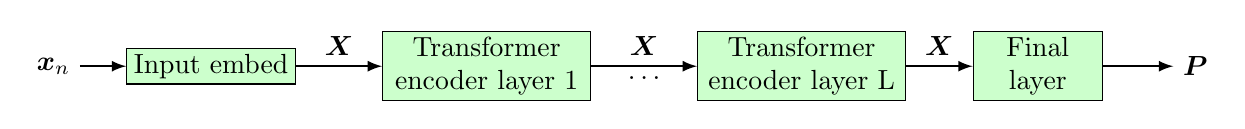
\begin{tikzpicture}
		
		\node (x) {$\bm{x}_n$};
		
		\node (emblayer) [param, right of=x, text centered, text width=2cm, xshift=1cm] {Input embed};
		
		%\node (X) [right of=emblayer, xshift=1cm] {$\bm{X}$};
		
		\node (trlayer1) [param, right of=emblayer, text centered, text width=2.5cm, xshift=2.5cm] {Transformer encoder layer 1};
		
		\node (trlayerN) [param, right of=trlayer1, text centered, text width=2.5cm, xshift=3cm] {Transformer encoder layer L};
		
		\node (finallayer) [param, right of=trlayerN, text centered, text width=1.5cm, xshift=2cm] {Final layer};
		
		\node (out) [right of=finallayer, xshift=1cm] {$\bm{P}$};
		
		\begin{scope}[thick, black, ->, >=latex]
			\draw (x) -- (emblayer);
			\draw (emblayer) -- (trlayer1) node [midway, above] {$\bm{X}$};
			\draw (trlayer1) -- (trlayerN) node [midway, above] {$\bm{X}$} node [midway, below] {$\ldots$};
			\draw (trlayerN) -- (finallayer) node [midway, above] {$\bm{X}$};
			\draw (finallayer) -- (out);
		\end{scope}	
	\end{tikzpicture}
	
	\vspace{4em}
	As usual, green boxes are functions with trainable parameters
	
\end{frame}	



\begin{frame}{BERT (encoding-only transformer, forward pass)}
	
	\begin{minipage}[t][3em][t]{15cm}
		\begin{algorithmic}[1]
			\Function{ETransformer}{$\bm{x} ; \bm{\mathcal{W}}$}
			\State $\ldots$
			\EndFunction
		\end{algorithmic}
		
	\end{minipage}
	
Input:

$\bm{x}$ --- $\bm{x} \in V^*$, a sequence of token IDs

$\bm{\mathcal{W}}$ --- all trainable parameters

Output:

Typically an embedding vector for each input token

Or: $\bm{P} \in (0,1)^{\ell_{\text{x}} \times N_{\text{V}}}$, where each row of $\bm{P}$ is a distribution over the vocabulary

\end{frame}




\begin{frame}{Input embeddings}
	
	The cat sat $\bm{x}_n =
	\begin{pmatrix}
		21 &
		11987 &
		5438
	\end{pmatrix}$
	
	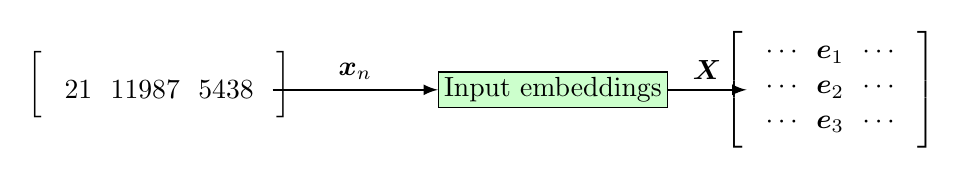
\begin{tikzpicture}
		
		\matrix[mtx, ampersand replacement=\&] (X) at (0,0) {
			21 \& 11987 \& 5438 \\
		};
		
		\node (embfn) [param, right of=X, xshift=4cm] {Input embeddings};
		
		\matrix[mtx,  ampersand replacement=\&, right=of embfn ] (embeddings) { 
			\cdots \& \bm{e}_1 \&  \cdots \\
			\cdots \& \bm{e}_2 \&  \cdots \\
			\cdots \& \bm{e}_3 \&  \cdots \\
			%		\cdots \& h_4 \&  \cdots \\
			%		\cdots \& h_5 \&  \cdots \\
		};
		
		\begin{scope}[thick, black, ->, >=latex]
			\draw (X) -- (embfn) node [midway, above] {$\bm{x}_n$};
			\draw (embfn) -- (embeddings) node [midway, above] {$\bm{X}$};
		\end{scope}	
	\end{tikzpicture}
\end{frame}	



\begin{frame}{BERT (encoding-only transformer, forward pass)}
	

\begin{minipage}[t][10cm][t]{15cm}
\begin{algorithmic}[1]
\Function{ETransformer}{$\bm{x} ; \bm{\mathcal{W}}$}
\State $\ell \gets \text{length}(\bm{x})$
\State for $t \in [\ell]: \bm{e}_t \gets \bm{W_e}[x[t],:] + \bm{W_p}[t,:]$
\Comment{Token emb. + positional emb.}
\State $\bm{X} \gets \text{Stack row-wise}[\bm{e}_1, \bm{e}_2, \ldots \bm{e}_{\ell}]$
\State $\ldots$
\EndFunction
\end{algorithmic}

\end{minipage}
\end{frame}



\begin{frame}{Transformer encoder (BERT)}
	
	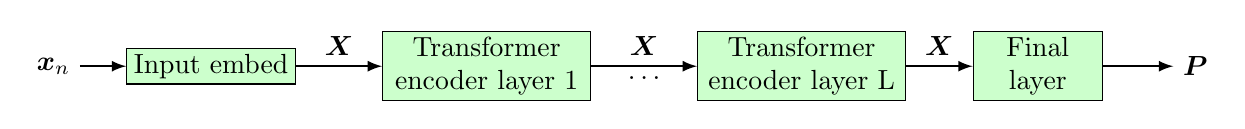
\begin{tikzpicture}
		
		\node (x) {$\bm{x}_n$};
		
		\node (emblayer) [param, right of=x, text centered, text width=2cm, xshift=1cm] {Input embed};
		
		%\node (X) [right of=emblayer, xshift=1cm] {$\bm{X}$};
		
		\node (trlayer1) [param, right of=emblayer, text centered, text width=2.5cm, xshift=2.5cm] {Transformer encoder layer 1};
		
		\node (trlayerN) [param, right of=trlayer1, text centered, text width=2.5cm, xshift=3cm] {Transformer encoder layer L};
		
		\node (finallayer) [param, right of=trlayerN, text centered, text width=1.5cm, xshift=2cm] {Final layer};
		
		\node (out) [right of=finallayer, xshift=1cm] {$\bm{P}$};
		
		\begin{scope}[thick, black, ->, >=latex]
			\draw (x) -- (emblayer);
			\draw (emblayer) -- (trlayer1) node [midway, above] {$\bm{X}$};
			\draw (trlayer1) -- (trlayerN) node [midway, above] {$\bm{X}$} node [midway, below] {$\ldots$};
			\draw (trlayerN) -- (finallayer) node [midway, above] {$\bm{X}$};
			\draw (finallayer) -- (out);
		\end{scope}	
	\end{tikzpicture}
	
	\vspace{4em}
	The transformer encoder layer is repeated L-times (each with different parameters)
	
\end{frame}	

\begin{frame}{BERT (encoding-only transformer, forward pass)}
	

\begin{minipage}[t][10cm][t]{15cm}
\begin{algorithmic}[1]
\Function{ETransformer}{$\bm{x} ; \bm{\mathcal{W}}$}
\State $\ell \gets \text{length}(\bm{x})$
\State for $t \in [\ell]: \bm{e}_t \gets \bm{W_e}[x[t],:] + \bm{W_p}[t,:]$
\Comment{Token emb. + positional emb.}
\State $\bm{X} \gets \text{Stack row-wise}[\bm{e}_1, \bm{e}_2, \ldots \bm{e}_{\ell}]$
\For{$l = 1, 2, \dots, L$}
\State $\ldots$
\EndFor
\EndFunction
\end{algorithmic}

	\end{minipage}
\end{frame}

\begin{frame}{Transformer encoder (BERT)}
	
	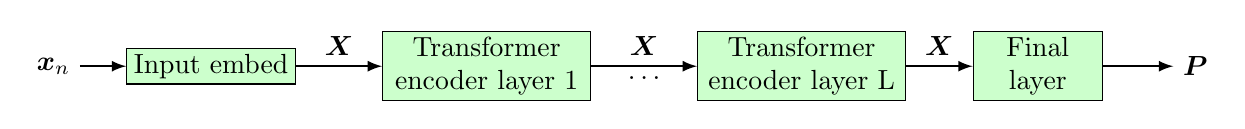
\begin{tikzpicture}
		
		\node (x) {$\bm{x}_n$};
		
		\node (emblayer) [param, right of=x, text centered, text width=2cm, xshift=1cm] {Input embed};
		
		%\node (X) [right of=emblayer, xshift=1cm] {$\bm{X}$};
		
		\node (trlayer1) [param, right of=emblayer, text centered, text width=2.5cm, xshift=2.5cm] {Transformer encoder layer 1};
		
		\node (trlayerN) [param, right of=trlayer1, text centered, text width=2.5cm, xshift=3cm] {Transformer encoder layer L};
		
		\node (finallayer) [param, right of=trlayerN, text centered, text width=1.5cm, xshift=2cm] {Final layer};
		
		\node (out) [right of=finallayer, xshift=1cm] {$\bm{P}$};
		
		\begin{scope}[thick, black, ->, >=latex]
			\draw (x) -- (emblayer);
			\draw (emblayer) -- (trlayer1) node [midway, above] {$\bm{X}$};
			\draw (trlayer1) -- (trlayerN) node [midway, above] {$\bm{X}$} node [midway, below] {$\ldots$};
			\draw (trlayerN) -- (finallayer) node [midway, above] {$\bm{X}$};
			\draw (finallayer) -- (out);
		\end{scope}	
	\end{tikzpicture}
	
	\vspace{4em}
	Let's look at a single transformer encoder layer
	
\end{frame}	

\begin{frame}{Transformer encoder layer (BERT)}
	
	\begin{tikzpicture}
		
		\node (X) {$\bm{X}$};
		
		\node (mhattention) [param, right of=X, text centered, text width=2cm, xshift=1cm, yshift=-1.6cm] {Multi-Head Self Attention};
		
		\node (sum1) [neuron, right of=X, text centered, text width=1.5cm, xshift=2.5cm] {Sum};
		
		\node (norm1) [param, right of=sum1, text centered, text width=1.5cm, xshift=1.5cm] {Layer Norm 1};
		
		\node (mlp1) [param, right of=norm1, text centered, text width=1.6cm, xshift=1.2cm, yshift=-1.4cm] {Linear layer 1};
		
		\node (gelu) [neuron, right of=norm1, text centered, text width=1.6cm, xshift=1.2cm, yshift=-2.6cm] {GELU};
		
		\node (mlp2) [param, right of=norm1, text centered, text width=1.6cm, xshift=1.2cm, yshift=-3.8cm] {Linear layer 2};
		
		\node (sum2) [neuron, right of=norm1, text centered, text width=1.5cm, xshift=2.8cm] {Sum};
		
		\node (norm2) [param, right of=sum2, text centered, text width=1.5cm, xshift=1.5cm] {Layer Norm 2};
		
		\node (out) [right of=norm2, xshift=1cm] {$\bm{X}$};		
		
		\begin{scope}[thick, black, ->, >=latex]
			\draw (x) edge[out=0,in=180] (mhattention);
			\draw (x) -- (sum1);
			\draw (mhattention) edge[out=0,in=270] (sum1) node [right of=mhattention, xshift=0.6cm, yshift=0cm] {$\bm{X}$};
			\draw (sum1) -- (norm1) node [midway, above] {$\bm{X}$};
			\draw (norm1) -- (sum2)  node [near start, above] {$\bm{X}$};
			\draw (norm1) edge[out=0,in=170] (mlp1);
			\draw (mlp1) -- (gelu);
			\draw (gelu) -- (mlp2);
			\draw (mlp2) edge[out=10,in=270] (sum2) node [right of=mlp2, xshift=0.3cm, yshift=0cm] {$\bm{X}$};
			\draw (sum2) -- (norm2) node [midway, above] {$\bm{X}$};
			\draw (norm2) -- (out);
		\end{scope}	
	\end{tikzpicture}

Let's focus on Multi-Head Self Attention	
\end{frame}


\begin{frame}{BERT (encoding-only transformer, forward pass)}

\vspace{-2em}
\begin{minipage}[t][10cm][t]{15cm}
\begin{algorithmic}[1]
\Function{ETransformer}{$\bm{x} ; \bm{\mathcal{W}}$}
\State $\ell \gets \text{length}(\bm{x})$
\State for $t \in [\ell]: \bm{e}_t \gets \bm{W_e}[x[t],:] + \bm{W_p}[t,:]$
\Comment{Token emb. + positional emb.}
\State $\bm{X} \gets \text{Stack row-wise}[\bm{e}_1, \bm{e}_2, \ldots \bm{e}_{\ell}]$
\For{$l = 1, 2, \dots, L$}
\State $\bm{X} \gets \bm{X} + \textsc{MHAttention}(\bm{X} | \bm{\mathcal{W}}_l)$
\Comment{Multi-head att., residual conn}
\State $\ldots$
\EndFor
\EndFunction
\end{algorithmic}

\end{minipage}
\end{frame}






\begin{frame}{Multi-head unmasked self-attention (BERT)}
	
	\begin{tikzpicture}
		
		\node (X) {$\bm{X}$};
		
		\node (ahead1) [param, right of=X, text centered, text width=2cm, xshift=2cm, yshift=1.6cm] {Attention head 1};
		
		\node (ahead2) [param, right of=X, text centered, text width=2cm, xshift=2cm, yshift=0cm] {Attention head 2};
		
		\node (aheadH) [param, right of=X, text centered, text width=2cm, xshift=2cm, yshift=-1.6cm] {Attention head H};
		
		\node (stack) [neuron, right of=ahead2, text centered, text width=1.5cm, xshift=2.5cm] {Stack};
		
		\node (linear) [param, right of=stack, text centered, text width=1.5cm, xshift=1.5cm] {Linear layer};
		
		\node (out) [right of=linear, xshift=1cm] {$\bm{X}$};		
		
		\begin{scope}[thick, black, ->, >=latex]
			\draw (x) edge[out=0,in=180] (ahead1);
			\draw (x) edge[out=0,in=180] (ahead2);
			\draw (x) edge[out=0,in=180] (aheadH);
			%			\draw (x) -- (sum1);
			\draw (ahead1) edge[out=0,in=170] (stack) node [right of=ahead1, xshift=0.5cm, yshift=0.4cm] {$\bm{Y}^1$};
			\draw (ahead2) edge[out=0,in=180] (stack) node [right of=ahead2, xshift=0.5cm, yshift=0.4cm] {$\bm{Y}^2$};
			\draw (aheadH) edge[out=0,in=190] (stack) node [right of=aheadH, xshift=0.5cm, yshift=0.7cm] {$\bm{Y}^H$};
			\draw (stack) -- (linear) node [midway, above] {$\bm{Y}$};
			%			\draw (norm1) -- (sum2)  node [near start, above] {$\bm{X}$};
			%			\draw (norm1) edge[out=0,in=180] (mlp);
			%			\draw (mlp) edge[out=0,in=270] (sum2) node [right of=mlp, xshift=0.3cm, yshift=0cm] {$\bm{X}$};
			%			\draw (sum2) -- (norm2) node [midway, above] {$\bm{X}$};
			\draw (linear) -- (out);
		\end{scope}	
	\end{tikzpicture}
	
\end{frame}



\begin{frame}{Multi-head bidirectional / unmasked self-attention}
	
\begin{minipage}[t][10cm][t]{15cm}

Input: $\bm{X} \in \mathbb{R}^{\ell_{\text{x}} \times d_{\text{x}}}$, vector representations of the sequence of length $\ell_{\text{x}}$

Output: $\bm{\tilde{V}} \in \mathbb{R}^{\ell_{\text{x}} \times d_{\text{out}}}$, updated vector representations of tokens in $\bm{X}$

Hyper-param: $H$, number of attention heads

Params for each $h \in [H]: \bm{\mathcal{W}_{qkv}}^h$:
\begin{itemize}
\item $\bm{W_q}^h, \bm{W_k}^h \in \mathbb{R}^{d_\text{x} \times d_\text{attn}}$,
$\bm{b_q}^h, \bm{b_k}^h \in \mathbb{R}^{d_\text{attn}}$,
$\bm{W_v} \in \mathbb{R}^{d_\text{x} \times d_\text{mid}}$, $ \bm{b_v} \in \mathbb{R}^{d_\text{mid}}$
\item $\bm{W_o} \in \mathbb{R}^{H \cdot d_\text{mid} \times d_\text{out}}$, $\bm{b_o} \in \mathbb{R}^{d_\text{out}}$	
\end{itemize}


\begin{algorithmic}[1]
\Function{MHAttention}{$\bm{X} ; \bm{\mathcal{W}}$}
\For{$h \in [H]$}
\State $\bm{Y}^h \gets \textsc{Attention}(\bm{X}; \bm{\mathcal{W}_{qkv}}^h)$
\Comment{$\bm{Y}^h \in \mathbb{R}^{\ell_{\text{x}} \times d_{\text{mid}}}}$
\EndFor
\State{$\bm{Y} \gets [\bm{Y}^1; \bm{Y}^2; \ldots; \bm{Y}^H]$}
\Comment{$\bm{Y} \in \mathbb{R}^{\ell_{\text{x}} \times H \cdot d_{\text{mid}}}}$
%\State $\bm{Q} \gets \bm{X} \bm{W_q} +_{\text{(rows)}} \bm{b_q}$
%\State $\bm{S} \gets \frac{1}{\sqrt{d_{\text{attn}}}} (\bm{Q} \bm{K}^\top)$
%\Comment{Scaled score $\in \mathbb{R}^{\ell_{\text{x}} \times \ell_{\text{x}}}$}
\State \Return $\bm{\tilde V} = \bm{Y} \bm{W_o} + \bm{b_o}$

\EndFunction
\end{algorithmic}

\end{minipage}
\end{frame}


\begin{frame}{Single unmasked self-attention head (BERT)}
	
	\begin{tikzpicture}
		
		\node (X) {$\bm{X}$};
		
		\node (query) [param, right of=X, text centered, text width=2.2cm, xshift=2cm, yshift=1.6cm] {Linear layer (query)};
		
		\node (key) [param, right of=X, text centered, text width=2.2cm, xshift=2cm, yshift=0cm] {Linear layer (key)};
		
		\node (value) [param, right of=X, text centered, text width=2.2cm, xshift=2cm, yshift=-1.6cm] {Linear layer (value)};
		
		\node (scaled) [neuron, right of=key, text centered, text width=1.5cm, xshift=2.5cm, yshift=1cm] {Scaled dot product};
		
		\node (softmax) [neuron, right of=scaled, text centered, text width=1.8cm, xshift=1.6cm] {Softmax (row)};
		
		\node (matmul) [neuron, right of=softmax, text centered, text width=1.5cm, xshift=1.5cm] {Matmul $\bm{\tilde{S}}\bm{V}$};
		
		\node (out) [right of=matmul, xshift=1cm] {$\bm{Y}^h$};		
		
		\begin{scope}[thick, black, ->, >=latex]
			\draw (x) edge[out=0,in=180] (query);
			\draw (x) edge[out=0,in=180] (key);
			\draw (x) edge[out=0,in=180] (value);
			%			\draw (x) -- (sum1);
			\draw (query) edge[out=0,in=170] (scaled) node [right of=query, xshift=0.5cm, yshift=0.4cm] {$\bm{Q}$};
			\draw (key) edge[out=0,in=190] (scaled) node [right of=key, xshift=0.5cm, yshift=0.4cm] {$\bm{K}$};
			\draw (value) edge[out=0,in=210] (matmul) node [right of=value, xshift=0.5cm, yshift=0.6cm] {$\bm{V}$};
			\draw (scaled) -- (softmax) node [midway, above] {$\bm{S}$};
			\draw (softmax) -- (matmul) node [midway, above] {$\bm{\tilde{S}}$};
			
			%			\draw (norm1) -- (sum2)  node [near start, above] {$\bm{X}$};
			%			\draw (norm1) edge[out=0,in=180] (mlp);
			%			\draw (mlp) edge[out=0,in=270] (sum2) node [right of=mlp, xshift=0.3cm, yshift=0cm] {$\bm{X}$};
			%			\draw (sum2) -- (norm2) node [midway, above] {$\bm{X}$};
			\draw (matmul) -- (out);
		\end{scope}	
	\end{tikzpicture}
	
\end{frame}


\begin{frame}{Bidirectional / unmasked self-attention (recap from last lecture)}
	
	\begin{minipage}[t][10cm][t]{15cm}
		
		Input: $\bm{X} \in \mathbb{R}^{\ell_{\text{x}} \times d_{\text{x}}}$, vector representations of the sequence of length $\ell_{\text{x}}$
		
		Output: $\bm{\tilde{V}} \in \mathbb{R}^{\ell_{\text{x}} \times d_{\text{out}}}$, updated vector representations of tokens in $\bm{X}$
		
		Params $\bm{\mathcal{W}_{qkv}}$: $\bm{W_q}, \bm{W_k} \in \mathbb{R}^{d_\text{x} \times d_\text{attn}}$, $\bm{b_q}, \bm{b_k} \in \mathbb{R}^{d_\text{attn}}$, $\bm{W_v} \in \mathbb{R}^{d_\text{x} \times d_\text{out}}$, $ \bm{b_v} \in \mathbb{R}^{d_\text{out}}$
		
		\begin{algorithmic}[1]
			\Function{Attention}{$\bm{X} ; \bm{\mathcal{W}_{qkv}}$}
			\State $\bm{Q} \gets \bm{X} \bm{W_q} +_{\text{(rows)}} \bm{b_q}$
			\Comment{Query $\in \mathbb{R}^{\ell_{\text{x}} \times d_{\text{attn}}}$}
			\State $\bm{K} \gets \bm{X} \bm{W_k} +_{\text{(rows)}} \bm{b_k}$
			\Comment{Key $\in \mathbb{R}^{\ell_{\text{x}} \times d_{\text{attn}}}$}
			\State $\bm{V} \gets \bm{X} \bm{W_v} +_{\text{(rows)}} \bm{b_v}$
			\Comment{Value $\in \mathbb{R}^{\ell_{\text{x}} \times d_{\text{out}}}$}
			
			\State $\bm{S} \gets \frac{1}{\sqrt{d_{\text{attn}}}} (\bm{Q} \bm{K}^\top)$
			\Comment{Scaled score $\in \mathbb{R}^{\ell_{\text{x}} \times \ell_{\text{x}}}$}
			
			\State \Return $\bm{\tilde V} = \softmax_{\text{row}}(\bm{S}) \bm{V}$
			
			\EndFunction
		\end{algorithmic}
		
	\end{minipage}
\end{frame}

\begin{frame}{Transformer encoder layer (BERT)}
	
	\begin{tikzpicture}
		
		\node (X) {$\bm{X}$};
		
		\node (mhattention) [param, right of=X, text centered, text width=2cm, xshift=1cm, yshift=-1.6cm] {Multi-Head Self Attention};
		
		\node (sum1) [neuron, right of=X, text centered, text width=1.5cm, xshift=2.5cm] {Sum};
		
		\node (norm1) [param, right of=sum1, text centered, text width=1.5cm, xshift=1.5cm] {Layer Norm 1};
		
		\node (mlp1) [param, right of=norm1, text centered, text width=1.6cm, xshift=1.2cm, yshift=-1.4cm] {Linear layer 1};
		
		\node (gelu) [neuron, right of=norm1, text centered, text width=1.6cm, xshift=1.2cm, yshift=-2.6cm] {GELU};
		
		\node (mlp2) [param, right of=norm1, text centered, text width=1.6cm, xshift=1.2cm, yshift=-3.8cm] {Linear layer 2};
		
		\node (sum2) [neuron, right of=norm1, text centered, text width=1.5cm, xshift=2.8cm] {Sum};
		
		\node (norm2) [param, right of=sum2, text centered, text width=1.5cm, xshift=1.5cm] {Layer Norm 2};
		
		\node (out) [right of=norm2, xshift=1cm] {$\bm{X}$};		
		
		\begin{scope}[thick, black, ->, >=latex]
			\draw (x) edge[out=0,in=180] (mhattention);
			\draw (x) -- (sum1);
			\draw (mhattention) edge[out=0,in=270] (sum1) node [right of=mhattention, xshift=0.6cm, yshift=0cm] {$\bm{X}$};
			\draw (sum1) -- (norm1) node [midway, above] {$\bm{X}$};
			\draw (norm1) -- (sum2)  node [near start, above] {$\bm{X}$};
			\draw (norm1) edge[out=0,in=170] (mlp1);
			\draw (mlp1) -- (gelu);
			\draw (gelu) -- (mlp2);
			\draw (mlp2) edge[out=10,in=270] (sum2) node [right of=mlp2, xshift=0.3cm, yshift=0cm] {$\bm{X}$};
			\draw (sum2) -- (norm2) node [midway, above] {$\bm{X}$};
			\draw (norm2) -- (out);
		\end{scope}	
	\end{tikzpicture}
	
	Let's add Layer Normalization and GELU	
\end{frame}


\begin{frame}{Simplifying notation: Perform \textsc{LayerNorm} on each row}
	
	\begin{block}{Recall: LayerNorm}
		Input: $\bm{e} \in \mathbb{R}^{d}$ (output of a layer), Output: $\bm{\hat e} \in \mathbb{R}^{d}$ \\
		Params: $\bm{\gamma}, \bm{\beta} \in \mathbb{R}^{d}$, trainable element-wise scale and offset
		
		\begin{algorithmic}[1]
			\Function{LayerNorm}{$\bm{e} | \bm{\gamma}, \bm{\beta}$}
			\State $m \gets \frac{1}{d} \sum_{i = 1}^{d} \bm{e}[i]$
			\Comment{`Sample mean' of $\bm{e}$}
			\State $v \gets \frac{1}{d} \sum_{i = 1}^{d} (\bm{e}[i] - m)^2$
			\Comment{`Sample variance' of $\bm{e}$}
			\State \Return $\bm{\hat e} = \frac{\bm{e} - m}{\sqrt{v}} \odot \bm{\gamma} + \bm{\beta}$
			\Comment{Offset and scale}
			\EndFunction
		\end{algorithmic}
	\end{block}
	
	
	\begin{algorithmic}[1]
		\Function{LayerNormEachRow}{$\bm{X} \in \mathbb{R}^{m \times n} | \bm{\gamma}, \bm{\beta}$}
		\For{$t \in [m]$}
		\State $˝\bm{X}[t,:] \gets \textsc{LayerNorm}(\bm{X}{[t,:]} | \bm{\gamma}, \bm{\beta})$
		\EndFor
		\State \Return $\bm{X}$
		\EndFunction
	\end{algorithmic}
	
	
\end{frame}



\begin{frame}{GELU --- Gaussian Error Linear Units}
	
	\begin{block}{Recall: CDF $\Phi(x)$ of standard normal $X \sim \mathcal{N}(0; 1)$}
		$\Phi(x) = \Pr(X \leq x) = \frac{1}{\sqrt{2 \pi}} \int_{-\infty}^{x} \exp \left(
		\frac{-t^2}{2} \right) \mathrm{d}t$
	\end{block}
	$$
	\begin{aligned}
		\textsc{GELU}(x) &= x \cdot \Phi(x) \\
		&\approx x \cdot \sigma(1.702 x) \qquad \text{(if speed $>$ exactness)}
	\end{aligned}
	$$
	
	\begin{figure}
		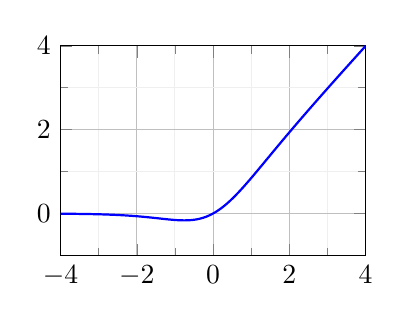
\begin{tikzpicture}
			
			\begin{axis}[
				xmin = -4, xmax = 4,
				ymin = -1, ymax = 4,
				xtick distance = 2,
				ytick distance = 2,
				grid = both,
				minor tick num = 1,
				major grid style = {lightgray},
				minor grid style = {lightgray!25},
				width = 0.45\textwidth,
				height = 0.35\textwidth,
				legend pos = north west
				]
				
				\addplot[
				domain = -10:10,
				samples = 200,
				smooth,
				thick,
				blue,
				] {
					x * 1/(1 + exp(-1 * 1.702 * x))
				};
				
			\end{axis}
		\end{tikzpicture}
	\end{figure}
	
	
	
	
	\begin{tikzpicture}[overlay, remember picture] 
		\node at (current page.north east)[ref] {\fullcite{Hendrycks.Gimpel.2016.arXiv} \newline \newline
			For vectors $\bm{x} \in \mathbb{R}^n$, $\textsc{GELU}(\bm{x})$ is applied element-wise
			\par};
	\end{tikzpicture}
	
	
\end{frame}





\begin{frame}{BERT (encoding-only transformer, forward pass)}

\vspace{-2em}
\begin{minipage}[t][10cm][t]{15cm}
\begin{algorithmic}[1]
\Function{ETransformer}{$\bm{x} ; \bm{\mathcal{W}}$}
\State $\ell \gets \text{length}(\bm{x})$
\State for $t \in [\ell]: \bm{e}_t \gets \bm{W_e}[x[t],:] + \bm{W_p}[t,:]$
\Comment{Token emb. + positional emb.}
\State $\bm{X} \gets \text{Stack row-wise}[\bm{e}_1, \bm{e}_2, \ldots \bm{e}_{\ell}]$
\For{$l = 1, 2, \dots, L$}
\State $\bm{X} \gets \bm{X} + \textsc{MHAttention}(\bm{X} | \bm{\mathcal{W}}_l)$
\Comment{Multi-head att., residual conn}
\State $\bm{X} \gets \textsc{LayerNormPerRow}(\bm{X} | \bm{\gamma^1}_l, \bm{\beta^1}_l)$
\State $\bm{X} \gets \bm{X} + \left(
\textsc{GELU}(\bm{X} \bm{W}^\text{mlp1}_l +_{\text{(row)}} \bm{b}^\text{mlp1}_l )
\bm{W}^{\text{mlp2}}_l +_{\text{(row)}} \bm{b}^{\text{mlp2}}_l \right)$
\Comment{MLP}
\State $\bm{X} \gets \textsc{LayerNormPerRow}(\bm{X} | \bm{\gamma^2}_l, \bm{\beta^2}_l)$
\EndFor
\State $\ldots$
\EndFunction
\end{algorithmic}

\end{minipage}
\end{frame}



\begin{frame}{Transformer encoder (BERT)}
	
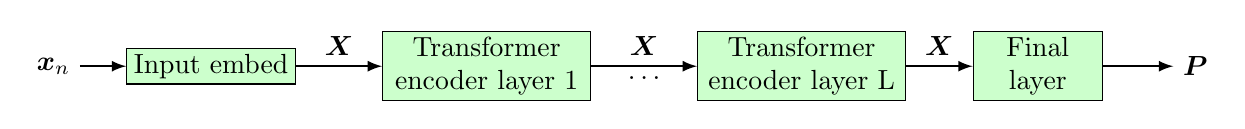
\begin{tikzpicture}

\node (x) {$\bm{x}_n$};

\node (emblayer) [param, right of=x, text centered, text width=2cm, xshift=1cm] {Input embed};

%\node (X) [right of=emblayer, xshift=1cm] {$\bm{X}$};

\node (trlayer1) [param, right of=emblayer, text centered, text width=2.5cm, xshift=2.5cm] {Transformer encoder layer 1};

\node (trlayerN) [param, right of=trlayer1, text centered, text width=2.5cm, xshift=3cm] {Transformer encoder layer L};

\node (finallayer) [param, right of=trlayerN, text centered, text width=1.5cm, xshift=2cm] {Final layer};

\node (out) [right of=finallayer, xshift=1cm] {$\bm{P}$};

\begin{scope}[thick, black, ->, >=latex]
	\draw (x) -- (emblayer);
	\draw (emblayer) -- (trlayer1) node [midway, above] {$\bm{X}$};
	\draw (trlayer1) -- (trlayerN) node [midway, above] {$\bm{X}$} node [midway, below] {$\ldots$};
	\draw (trlayerN) -- (finallayer) node [midway, above] {$\bm{X}$};
	\draw (finallayer) -- (out);
\end{scope}	
\end{tikzpicture}

\vspace{4em}
Let's look at the final layers

\end{frame}	



\begin{frame}{Final layer (BERT)}
	
	\begin{tikzpicture}
		
		\node (X) {$\bm{X}$};
		
		\node (linear) [param, right of=X, text centered, text width=1.5cm, xshift=1.5cm] {Linear layer};
		
		\node (gelu) [neuron, right of=linear, text centered, text width=1.5cm, xshift=1.5cm] {GELU};
		
		\node (norm) [param, right of=gelu, text centered, text width=1.5cm, xshift=1.5cm] {Layer Norm};
		
		\node (out) [right of=norm, xshift=1cm] {$\bm{Z}$};
		
		\node (linear2) [param, below of=linear, text centered, text width=1.5cm, yshift=-1.5cm] {Linear layer};
		
		\node (softmax) [neuron, right of=linear2, text centered, text width=1.8cm, xshift=1.5cm] {Softmax (row)};
		
		\node (out2) [right of=softmax, xshift=1cm] {$\bm{P}$};
		
		\begin{scope}[thick, black, ->, >=latex]
			\draw (x) -- (linear);
			\draw (linear) -- (gelu);
			\draw (gelu) -- (norm);
			\draw (norm) -- (out);
			\draw (out) edge[out=270,in=90, dotted] (linear2) node [right of=linear2, xshift=0.5cm, yshift=1.1cm] {unembedding};
			\draw (linear2) -- (softmax);
			\draw (softmax) -- (out2);
		\end{scope}
	\end{tikzpicture}
	
\end{frame}

\begin{frame}{BERT (encoding-only transformer, forward pass)}
	
	\vspace{-2em}
	\begin{minipage}[t][10cm][t]{15cm}
		\begin{algorithmic}[1]
			\Function{ETransformer}{$\bm{x} ; \bm{\mathcal{W}}$}
			\State $\ell \gets \text{length}(\bm{x})$
			\State for $t \in [\ell]: \bm{e}_t \gets \bm{W_e}[x[t],:] + \bm{W_p}[t,:]$
			\Comment{Token emb. + positional emb.}
			\State $\bm{X} \gets \text{Stack row-wise}[\bm{e}_1, \bm{e}_2, \ldots \bm{e}_{\ell}]$
			\For{$l = 1, 2, \dots, L$}
			\State $\bm{X} \gets \bm{X} + \textsc{MHAttention}(\bm{X} | \bm{\mathcal{W}}_l)$
			\Comment{Multi-head att., residual conn}
			\State $\bm{X} \gets \textsc{LayerNormPerRow}(\bm{X} | \bm{\gamma^1}_l, \bm{\beta^1}_l)$
			\State $\bm{X} \gets \bm{X} + \left(
			\textsc{GELU}(\bm{X} \bm{W}^\text{mlp1}_l +_{\text{(row)}} \bm{b}^\text{mlp1}_l )
			\bm{W}^{\text{mlp2}}_l +_{\text{(row)}} \bm{b}^{\text{mlp2}}_l \right)$
			\Comment{MLP}
			\State $\bm{X} \gets \textsc{LayerNormPerRow}(\bm{X} | \bm{\gamma^2}_l, \bm{\beta^2}_l)$
			\EndFor
			\State $\bm{X} \gets \textsc{GELU}(\bm{X} \bm{W_f}  +_{\text{(row)}} \bm{b_f} )$
			\State $\bm{X} \gets \textsc{LayerNormPerRow}(\bm{X} | \bm{\gamma}_l, \bm{\beta}_l)$
			\State \Return $\bm{P} = \softmax(\bm{X} \bm{W_u}) $
			\Comment{Project to vocab., probabilities}
			\EndFunction
		\end{algorithmic}
		
	\end{minipage}
\end{frame}



\begin{frame}{BERT parameters and hyperparameters}
	
	\begin{minipage}[t][10cm][t]{15cm}
			
		Hyperparameters: $\ell_{\text{max}}, L, H, d_{\text{e}}, d_{\text{mlp}}, d_{\text{f}} \in \mathbb{N}$
		
		Parameters:
		
		$\bm{W_e} \in \mathbb{R}^{N_\text{V} \times d_\text{e}}$, $\bm{W_p} \in \mathbb{R}^{\ell_{\text{max}} \times d_\text{e}}$, the token and positional embedding matrices
		
		For $l \in [L]: \bm{\mathcal{W}}_l$, multi-head attention parameters for layer $l$:
		
		\begin{itemize}
		\item $\bm{\gamma^1}_l, \bm{\beta^1}_l, \bm{\gamma^2}_l, \bm{\beta^2}_l$, two sets of layer-norm parameters
		\item $\bm{W}^{\text{mlp1}}_l \in \mathbb{R}^{d_{\text{e}} \times d_\text{mlp}}$, $\bm{b}^{\text{mlp1}}_l \in \mathbb{R}^{d_\text{mlp}}$
		\item $\bm{W}^{\text{mlp2}}_l \in \mathbb{R}^{d_\text{mlp} \times d_{\text{e}}}$, $\bm{b}^{\text{mlp2}}_l \in \mathbb{R}^{d_\text{e}}$
		\end{itemize}
		
		
		
		
		$\bm{W_f} \in \mathbb{R}^{d_\text{e} \times d_\text{f}}, \bm{b_f} \in \mathbb{R}^{d_\text{f}}$, $\bm{\gamma},\bm{\beta} \in \mathbb{R}^{d_\text{f}}$, the final linear projection and layer-norm parameters.
		
		
		$\bm{W_u} \in \mathbb{R}^{d_\text{e} \times N_\text{V}}$, the unembedding matrix
		
	\end{minipage}
\end{frame}

\section{Input and pre-training}

\begin{frame}{BERT: Tokenization}
	
	Tokenizing into a multilingual WordPiece inventory
	
	\begin{itemize}
		\item Recall that WordPiece units are sub-word units
		\item 30,000 WordPiece units (newer models 110k units, 100 languages)
	\end{itemize}
	
	Implications: BERT can "consume" any language
	
	
\end{frame}


\begin{frame}{BERT: Input representation}
	
	\begin{itemize}
		\item Each WordPiece token from the input is represented by a \textbf{WordPiece embedding} (randomly initialized)
		\item Each position from the input is associated with a \textbf{positional embedding} (also randomly initialized)
		\item Input length limited to \textbf{512} WordPiece tokens, using \texttt{<PAD>}ding
		\item Special tokens
		\begin{itemize}
			\item The fist token is always a special token \textbf{[CLS]}
			\item If the task involves two sentences (e.g., NLI), these two sentences are separated by a special token \textbf{[SEP]}; also special two \textbf{segment position embeddings} 
		\end{itemize}
		
	\end{itemize}
	
\end{frame}


\section{Pre-training}





\begin{frame}{BERT: Pre-training data generation}
	
	Take the entire Wikipedia (in 100 languages; 2,5 billion words)
	
	To generate a single training instance, sample two segments (max combined length 512 WordPiece tokens)
	
	\begin{itemize}
		\item For Task 2, replace the second segment randomly in 50\% (negative samples)
		\item For Task 1, choose random 15\% of the tokens, and in 80\% replace with a [MASK] 
	\end{itemize}
	
	
\end{frame}



\begin{frame}{BERT: pre-training by masked language modeling}
	
	\vspace{-1em}	
	\begin{minipage}[t][10cm][t]{15cm}
		\begin{algorithmic}[1]
			\Function{ETraining}{$\left\{ \bm{x}_n \right\}_{n = 1}^{N_\text{data}}$ seqs,  $\bm{\theta}$ init.\ params; $p_{\text{mask}} \in (0, 1)$, $N_\text{epochs}$, $\eta$}
			\For{$i \in [N_{\text{epochs}}]$}
			\For{$n \in [N_{\text{data}}]$}
			\State $\ell \gets \text{length}(\bm{x}_n)$
			\For{$t \in [\ell]$}
			\State $\tilde{\bm{x}}_n[t] \gets \texttt{<mask\_token>}$ with prob.\ $p_{\text{mask}}$, otherwise $\bm{x}_n[t]$
			\EndFor
			\State $\tilde{T} \gets \left\{ t \in [\ell] : \tilde{\bm{x}}_n[t] = \texttt{<mask\_token>} \right\}$
			\Comment{Indices of masked tokens}
			\State $\bm{P_{\theta}} \gets \textsc{ETransformer}(\tilde{\bm{x}}_n | \bm{\theta})$
			\State $\text{loss}_{\bm{\theta}} \gets - \sum_{t \in \tilde{T}} \log \bm{P_{\theta}} [t, \bm{x}_n[t]] $
			\State $\bm{\theta} \gets \bm{\theta} - \eta \cdot \nabla \text{loss}_{\bm{\theta}}$
			\EndFor
			\EndFor
			\State \Return $\bm{\theta}$
			\EndFunction
		\end{algorithmic}
		
	\end{minipage}
\end{frame}




\begin{frame}{Simple example explaining lines 6--7 (masking)}
	$
	\begin{pmatrix}
		\text{The} &
		\text{cat} &
		\text{sat}
	\end{pmatrix}
	\rightarrow
	\bm{x}_n =
	\begin{pmatrix}
		21 &
		11987 &
		5438
	\end{pmatrix}
	\quad \text{(Indices in $V$)}
	$
	
	Random masking (index of \texttt{<mask\_token>} = 50001):
	\begin{enumerate}
		\item For $t = 1$, the random outcome is "mask"
		\item For $t = 2$, the random outcome is "keep"
		\item For $t = 3$, the random outcome is "mask"
	\end{enumerate}
	$
	\bm{\tilde{x}}_n =
	\begin{pmatrix}
		50001 &
		11987 &
		50001
	\end{pmatrix},
	\tilde{T} = \left\{ 1, 3 \right\}
	$
	
	
	
\end{frame}



\begin{frame}{Explaining line 9 (negative log likelihood)}
	
	$
	\begin{pmatrix}
		\text{The} &
		\text{cat} &
		\text{sat}
	\end{pmatrix}
	\rightarrow
	\bm{x}_n =
	\begin{pmatrix}
		21 &
		11987 &
		5438 
	\end{pmatrix},
	\bm{\tilde{x}}_n =
	\begin{pmatrix}
		50001 &
		11987 &
		50001
	\end{pmatrix},
	\tilde{T} = \left\{ 1, 3 \right\}
	$
	
	$\bm{P_{\theta}} \gets \textsc{ETransformer}(\tilde{\bm{x}}_n | \bm{\theta})$
	$$
	\bm{P_{\theta}} =
	\begin{pmatrix}
		0.001 & 0.0007 & \ldots & 0.0003 \\
		0.0013 & 0.0065 & \ldots & 0.0001 \\
		0.079 & 0.015 & \ldots & 0.0001 \\
	\end{pmatrix}
	$$
	
	$\bm{P_{\theta}} \in (0,1)^{\ell_{\text{x}} \times N_{\text{V}}}$, where each row of $\bm{P}$ is a distribution over the vocabulary
	
\end{frame}


\begin{frame}{Explaining line 9 (negative log likelihood), $t = 1$}
	
	\begin{small}
		$\bm{x}_n = (21, 11987, 5438), \bm{\tilde{x}}_n = (50001, 11987, 50001), \tilde{T} = \left\{ 1, 3 \right\}$
		
		$
		\bm{P_{\theta}} =
		\begin{pmatrix}
			0.001 & \ldots & 0.0041_{21} & \ldots 0.0003 \\
			\vdots &  &  &  \\
		\end{pmatrix}
		$
	\end{small}	
	
	For $t = 1$, the model should learn to predict "The" (index 21)
	
	Gold: $\bm{y} = (0, 0, \ldots, 1_{21}, \ldots, 0) \in \mathbb{R}^{N_{\text{V}}}$
	
	Pred: $\bm{\hat{y}} = \bm{P_{\theta}}[1,:] = (0.001, \ldots, 0.0041_{21}, \ldots 0.0003) \in \mathbb{R}^{N_{\text{V}}}$
	
	\begin{block}{Categorical cross entropy loss (Lec.\ 4)}
		$L (\bm{\hat{y}, \bm{y}}) := - \sum_{k = 1}^{K} \bm{y}_{[k]} \log \left(  \bm{\hat{y}}_{[k]} \right)$ \\
		$= - 1 \cdot \log (\bm{\hat{y}}[21])
		= - \log(\bm{P_{\theta}}[1, 21])$ \\
		$= - \log(\bm{P_{\theta}}[1, \bm{x}_n[1]]) 
		= - \log(\bm{P_{\theta}}[t, \bm{x}_n[t]])$	
	\end{block}
	
\end{frame}


\begin{frame}{Explaining line 9 (negative log likelihood), $t = 3$}
	
	\begin{small}
		$\bm{x}_n = (21, 11987, 5438), \bm{\tilde{x}}_n = (50001, 11987, 50001), \tilde{T} = \left\{ 1, 3 \right\}$
		
		$
		\bm{P_{\theta}} =
		\begin{pmatrix}
			\vdots &  \cdots &  \cdots &  \\
		\end{pmatrix}
		$
	\end{small}	
	
	For $t = 3$, the model should learn to predict "sat" (id 5438)
	
	\begin{block}{Categorical cross entropy loss}
		$L (\bm{\hat{y}, \bm{y}}) := - \sum_{k = 1}^{K} \bm{y}_{[k]} \log \left(  \bm{\hat{y}}_{[k]} \right)$ \\
		$= - 1 \cdot \log (\bm{\hat{y}}[5438])
		= - \log(\bm{P_{\theta}}[3, 5438])
		= - \log(\bm{P_{\theta}}[t, \bm{x}_n[t]])$	
	\end{block}
	
	
	Sum over all masked token positions in $\tilde{T}$ gives us line 9:\\
	$$\text{loss}_{\bm{\theta}} \gets - \sum_{t \in \tilde{T}} \log \bm{P_{\theta}} [t, \bm{x}_n[t]] $$
	
\end{frame}







\section{Downstream tasks and fine-tuning}





\begin{frame}{BERT pre-training time}
		
	Pretraining BERT took originally 4 days on 64 TPUs\footnote{Can be done more efficiently, see, e.g., \citet{izsak-etal-2021-train}}
	
	\bigskip
	
	Once pre-trained, transfer and "fine-tune" on your small-data task and get competitive results


	
\begin{tikzpicture}[overlay, remember picture] 
	\node at (current page.north east)[ref] {\fullcite{izsak-etal-2021-train} \par};
\end{tikzpicture}

	
\end{frame}


\begin{frame}{Recap}
	
	BERT stays on the shoulders of many clever concepts and techniques, mastered into a single model
	
\textbf{What do we know about how BERT works?}

	
\emph{``BERTology has clearly come a long way, but it is fair to say we still have more questions than answers about how BERT works.''} --- \citet{Rogers.et.al.2020.BERT}\footnote{Highly recommended reading!}
	
	
\begin{tikzpicture}[overlay, remember picture] 
	\node at (current page.north east)[ref] {\fullcite{Rogers.et.al.2020.BERT} \par};
\end{tikzpicture}
	
\end{frame}











	







\begin{frame}{License and credits}

	\begin{columns}
		\begin{column}{0.7\textwidth}
			Licensed under Creative Commons Attribution-ShareAlike 4.0 International (CC BY-SA 4.0)
		\end{column}
		\begin{column}{0.2\textwidth}
			
\includegraphics[width=0.9\linewidth]{img/cc-by-sa-icon.pdf}
		\end{column}
	\end{columns}
	
	\bigskip
	
	Credits
	
	\begin{scriptsize}
		
		Ivan Habernal
		
		Content from ACL Anthology papers licensed under CC-BY \url{https://www.aclweb.org/anthology}
		
	
	\end{scriptsize}
	
\end{frame}



\end{document}

